\documentclass[12pt]{article}
\usepackage{amsmath}
\usepackage{graphicx}
\usepackage{hyperref}
\usepackage{xcolor}

\addtolength{\oddsidemargin}{-.875in}
\addtolength{\evensidemargin}{-.875in}
\addtolength{\textwidth}{1.75in}

\addtolength{\topmargin}{-.875in}
\addtolength{\textheight}{1.75in}

\title{Model Predictive Control}
\date{2019}
\author{author}

\begin{document}
\pagecolor{gray}
\maketitle
\section{Introduction}
This note documents the Model Predictive Control (MPC) method for the two
wheel balancing robot. Many people has built similar self-balancing robots.
Almost all of them uses PID control as the control strategy. For position
estimation, some uses Kalman filters, and others uses complementary filters.

The purpose of using MPC in this robot is not trying to invent a new MPC
technique, which usually the case for research papers.
But rather I intend to 1) practice MPC and 2) test how well MPC behaves
compares to other control schemes.

\section{Robot Coordinates}
As shown in Figure~\ref{fig_coordinates}, $\theta_k$ and $\omega_k$ denotes 
the angular position at time step $k$, respectively.
Counter-clockwise rotation is positive. $u_k$ is the linear wheel velocity
with positive to the right. Robot specifications can be found in 
Table~\ref{tab_robot_specification}


\begin{figure}[h]
  \label{fig_coordinates}
  \centering
  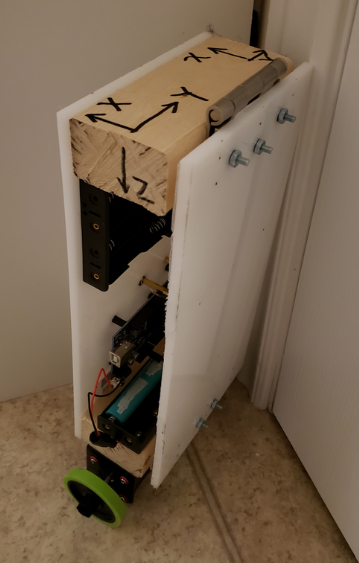
\includegraphics[scale=0.5]{./figures/coordinates.png}
  \caption{Robot Coordinates}
\end{figure}

\begin{table}
  \centering
  \begin{tabular}{l|c|c}
    \hline
	Specification & Notation & Value \\ \hline
    Center of Gravity (CoG) & $h$ & ?? 0.2m \\ 
	Mass & $m$ & ?? 1.1kg \\ \hline
  \end{tabular}
  \caption{Robot specification} 
  \label{tab_robot_specification}
\end{table}


\section{Problem Formulation}
The model is a 1-input-2-output model.

\begin{align}
\label{equ_orig_nonlinear_dynamics}
x_{k+1} & = f(x_k, u_k) \\
y_k & = C(x_k)x_k
\end{align}

$x_k=[\theta_k\,\,\,\omega_k]^T$ is the system state. 
Linearize Equ~\ref{equ_orig_nonlinear_dynamics}, we have

\begin{align}
x_{k+1} & = A(x_k)x_k + B(x_k)u_k \\
y_k & = C(x_k)x_k
\end{align}

where 

\begin{align}
A(x_k) = \frac{\partial f}{\partial x_k},
B(x_k) = \frac{\partial f}{\partial u_k}
\end{align}

\end{document}
%
%
%
%
%
%
%
%
%
%
%
%
%
%
%
%
